\documentclass[a4paper]{article}
\usepackage{graphicx}
\usepackage[bookmarks=true]{hyperref}
\usepackage{bookmark}
\usepackage[margin=1.2in]{geometry}
\usepackage{float}
\usepackage{caption}
\usepackage{hyperref}
\usepackage[english]{babel}
\usepackage{graphicx}

\title{Architectural Requirements}
\author{The Baobab Team}

\begin{document}

\newpage
\begin{titlepage}

\begin{center}


\includegraphics[width=400px]{pictures/logo.jpg}
\vspace{0.5 cm}
\begin{flushright} \large
\begin{tabular}{lr}
\vspace{1 cm}
\LARGE\textbf{Document:}Sprint Report 6\\

\vspace{1 cm}
\LARGE\textbf{Project:} Group Chat For Linphone (Agile DO-178)\\
\vspace{1 cm}
\LARGE\textbf{Advisor:} Kobus Coetzee\\
\vspace{1 cm}
\LARGE\textbf{Sponsors:} Nanoteq \& Department of Computer Science, UP\\
\vspace{1 cm}
\LARGE\textbf{Date: }\today\\
\end{tabular}
\end{flushright}

\centering 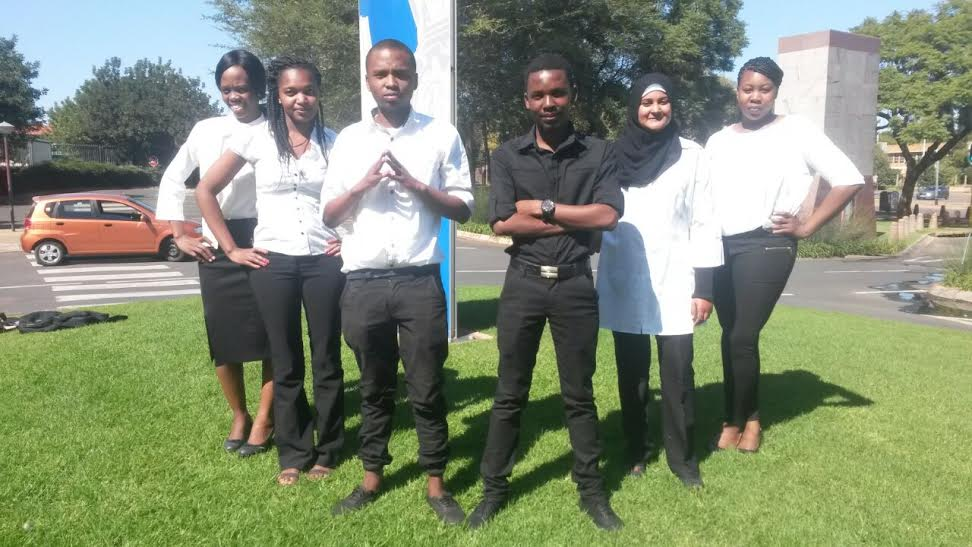
\includegraphics[width=350px]{pictures/Team.jpg}

Patience Mtsweni, Lerato Molokomme, Tsepo Ntsaba, Mpedi Mello, Lutfiyya Razak, Ephiphania Munava\\


\end{center}
\end{titlepage}

\newpage
\begin{center}
\LARGE \textbf{Member details}\\
\begin{tabular}{ll}
Ephiphania Munava&10624610\\
Lutfiyya Razak&10198408\\
Lerato Molokomme&11197961\\
Mpedi Mello&11210754\\
Patience Mtsweni&11116774\\
Tsepo Ntsaba&10668544\\

\end{tabular}
\end{center}

\newpage

\tableofcontents

\newpage

\section{\textbf{Introduction}}
The purpose of this project is to extend Linphone's Instant Messaging (IM) implementation on Android platforms to include group chat and to implement other minor improvements to Linphones IM capabilities and user interface.
\section{\textbf{Scope}}
We are required to develop the following functionality for the Linphone project:
\begin{itemize}
\item Group chat (Invite additional members to a chat, all members receive chats)
\item Secure group chat (AES256)
\item Creation and deletion of groups
\item Voice record and send over IM
\item Improve the messaging user interface
	\begin{itemize}
		\item Spacing between words are terrible
		\item Make text bigger
		\item Blocks indents required to better specify who said what
		\item Presence indication to show a remote user is typing
		\item User picture portraits
	\end{itemize}
\end{itemize}

\section{\textbf{Access and Integration Channel}}
	\subsection{Access Channels}
	\subsubsection{Human access channels}
	The system will be accessible by human users through the following channels:
	\begin{itemize}
	\item Android devices
	\end{itemize}

	\subsubsection{System access channels}
	Linphone provides a library called Liblinphone which is a cross-platform SDK for SIP communication and media processing. It's an easy to use API, that enables other systems such as iOS, Blacberry, Windows phone, Linux, Mac and windows to have access to the system.
	
	
	\subsection{Integration channels}
	The system will be able to access the following for chat purposes:
	\begin{itemize}
	\item Phonebook contacts
	\item Pictures
	\item Videos
	\item Sound
	\end{itemize}
	
	
	%%%%%%%%%%% Architectural requirements %%%%%%%%%%%
\section{\textbf{Architecture Requirements}}

\subsection{Architectural Scope}
\begin{itemize}	
		\item Platform independent
			\begin{itemize}
				\item The system is accessible on the website however the group chat functionality will be accessible implemented is only for a android mobile application.
			\end{itemize}
\end{itemize}

\begin{itemize}	
		\item Distributed databases
			\begin{itemize}
				
				\item We are making use of the Linphone database to store the messages.
			\end{itemize}
\end{itemize}

\begin{itemize}	
		\item Security
			\begin{itemize}
				\item Confidentiality: Encrypt messages when users are chatting		
			\end{itemize}
			
		\item Backup
		  \begin{itemize}
			  \item The system should run on multiple servers.
			  \item The system should have an automated database backup.
			  \item The system should have alternative platforms(i.e. smart phones, etc.).
		  \end{itemize}					
		  
		\item Store uploaded content (i.e. docs, images)
		  \begin{itemize}
			  \item The system should allow the user to be able to upload an image should they wish to.
		  \end{itemize}					
		
\end{itemize}

\subsection{Quality Requirements}
\subsubsection{Usability}
Usability is an important quality requirement needed by the system. Usability takes first priority over other quality requirements. We divide usability into this :\\

\begin{itemize}
\item \textbf{Learnability} \\
The interface should be designed in such a way that it is easy to use and learn. If the user is a first time user then the system should not be hard to understand. 
The interface should not be complex for the user, it should include basic functions and fewer things to learn and remember.

\item \textbf{Error Handling} \\
The system should be able to handle errors made by users. Correct, prevent or even detect them. If there is no group name entered it will let the user know before it moves to the next screen.
Users will be allowed to perform certain operations based on their user level. Some functions will be deactivated for certain users. 
For example a member cannot removed other members from the group, only the administrator can do that. Such functionality will be hidden from the user preventing errors. 

\item \textbf{Acceptability} \\
Acceptability is a subjective phenomenon to which many factors contribute, it measures the extent to which users like the system. 
The system should be created in such a way that the users are comfortable with and they actually like it, this can be achieved by a technique called Usability Testing where we have users that test our system and get feedback from them by giving them questionnaires which will require answers based on the system they interacted with.


\item \textbf{Effectiveness} \\
The system should be effective in such a way that it does the right tasks, completing activities and achieving the required goals. It should allow users to exchange messages in a group and send voice recording.
\end{itemize}

\subsubsection{Security}
Security is an important issue in the group chat. A Secure system focuses on three main aspects, namely: to detect attacks, resist attacks and recover from attacks.\\
We will, however on the Linphone group chat focus on the resisting attacks. The messages that are exchanged in the group chat will be encrypted before being sent and minutes to discourage bot attacks, this might, however, have an impact on usability.\\

\subsubsection{Availability}
The system must to be available when needed by the users and by the members of a group chat for communicating\\

\subsubsection{Reliability}
The system should be reliable in such a way that it will be easy to implement or make changes on it should any errors or failures occur, the system should be able to handle them and recover easily.\\	
	

\section{\textbf{Architectural Tactics or Strategies}}

\subsection{Maintainability}

In order to improve maintainability and reduce the skills requirements for the team who needs to maintain the system, the software architecture of the system has been split into submodules, which allows for flexibility and easy maintainability because a dedicated team will be in charge of a specific submodule. This allows for automatic updating, if the submodules are update, the system will automatically upgrade the source code for future downloads.

\subsection{Reliability and Availability}

Linphone is hosted by Belldone communications, thus it is hosted privately even though it is open source, thus ensuring that it will always be available and reliable.

\subsection{Security}

There are a number of tactics we are using to ensure security. The first is authentication, a user has to register and be authenticated to chat using Linphone. Further security measures we implemented are that we are using the ZRTP protocol to encrypt voice calls. We are also using the ORT protocol to encrypt the instant messages and to ensure no third parties can eaves drop on a conversation. We are also using the Socialist Millionaire Protocol to detect man in the middle attacks and eaves dropping.

\subsection{Testability}

Continuous Integration and Development is a agile tactic that we are using for ensuring that we test the code efficiently. We also use unit tests to test the code based on the service contracts.

\subsection{Usability}

The user interface has been separated from the rest of the application. Since the user interface is expected to change frequently both during the development and after development, maintaining the user interface code separately will localize changes to it. Usability can only be achieved through rigorous testing and modification, satisfying the HCI components such as error handling and proper feedback when a user clicks on a button etc. Using templates has also been used to enforce a consistent user interface and maintainability.

\subsection{Intergrability}

Since Linphone has a modular design, meaning it has been subdivided into smaller parts called modules or submodules it is easy to integrate new submodules and functionalities.

Since we are also using continuous integration, which means merging several developers’ code in to the mainline several times a day, to solve integration problems.


\section{\textbf{Architectural Components}}

\subsection{LibLinphone}

Liblinphone is a high level library integrating all the SIP video calls feature into a single easy to use API. Usually telecommunications is made of two things: media (transport of voice or video, encoding and decoding), and signalling (routing calls, ringing, accepting a call).
Liblinphone aims at combining the two things together and doing most things automatically. This makes it easier to the programmer to implement video calls in any application, without being an expert in VoIP and telecommunications. Liblinphone is an open source library based on Mediastreamer2 for voice/video streaming, and belle-sip for SIP signalling.

\subsection{Mediastreamer2}

Mediastreamer2 is a powerful and lightweight streaming engine specialized for voice/video telephony applications.
This open source library is responsible for all the receiving and sending of multimedia streams in Linphone, including voice/video capture, encoding and decoding, and rendering.

\subsection{Belle-SIP}

Belle-sip is a C object oriented SIP Stack.

\subsection{ORTP}

oRTP is a library implementing Real-time Transport Protocol (RFC3550), licensed under LGPL.

\subsection{Bcg729}

Bcg729 is a software G729A encoder and decoder library written in C, developed by Belldone communications, the company supporting the Linphone project. It was written from scratch and is NOT a derivative work of ITU reference source code in any kind.
It can be executed on many platforms, including both ARM and x86 with very decent performances. Libbcg729 supports concurrent channel encoding/decoding for multi-call applications such as conferencing.
The source code also contains a mediastreamer2 compatible plugin, designed for use of this codec in Linphone or mediastreamer2-based software. However a direct API is available for those not using bcg729 with mediastreamer2.

\subsection{Flexisip}

Flexisip is a SIP proxy server implementation compliant to RFC3261.
The project was started by Belldone Communications in 2011. The focus was to develop a SIP proxy solution easy to install, configure and maintain, and offering “out of the box” all the required features to deploy a SIP service tuned for mobile applications.
The free linphone.org SIP service is running with Flexisip since 2011, and enables Linphone users to create their SIP addresses in order to communicate together.
Thanks to its modular architecture and its limited number of required dependencies, Flexisip can perfectly run on small hardware’s (embedded systems).

\section{Technologies}
\begin{itemize}
\item For version control, we are using github. It has our git repository, which has a branch for each feature or bug. The branches are only merged with the main trunk once it passes the unit test and travis-ci for th continuous integration\\
\item IDE we are using is Eclipse\\
\item We are using travis-ci for builds. It is used for building and performing continuous integration or Continuous deployment. If the build fails then we do not merge the new feature or bug fix with the main trunk until it can build with Travis which is linked with our git repository.\\
\item We are using Trello for our scrum board, where there is our product backlog with all our user stories to be implemented, it has the sprint backlog for each sprint, it has a list of completed user stories and those that still need to be completed.\\
\item The group chat user interface is coded in java (Android) and for unit test, JUnit is used\\
\item The group chat back-end functionality is coded in C and for unit testing, CUnit is used.

\end{itemize}

\section{References}
\begin{itemize}
\item Linphone information, Avaiable from: https://www.linphone.org [Accessed: 28 August 2015]
\end{itemize}

\end{document}